\subsection{Pitch Generation}\label{subsec:Pitch_Generation}

Die Hauptaufgabe der Komponente Pitch Generation ist es das Audiosignal aus dem Rechtecksignal der Tonhöhenantenne (Pitch Antenna) zu generieren. Pitch Generation nimmt zudem eine Frequenzmessung des Audiosignals vor um diverse Funktionalitäten zu gewährleisten. In Abbildung \ref{img:Blockschaltbild_pitch} ist der Grobe aufbau der Komponente aufgezeigt. Die genaue Erklärung zu den einzelnen Komponenten ist in den folgenden Abschnitten zu finden.


\begin{figure}[h!]
	\centering
	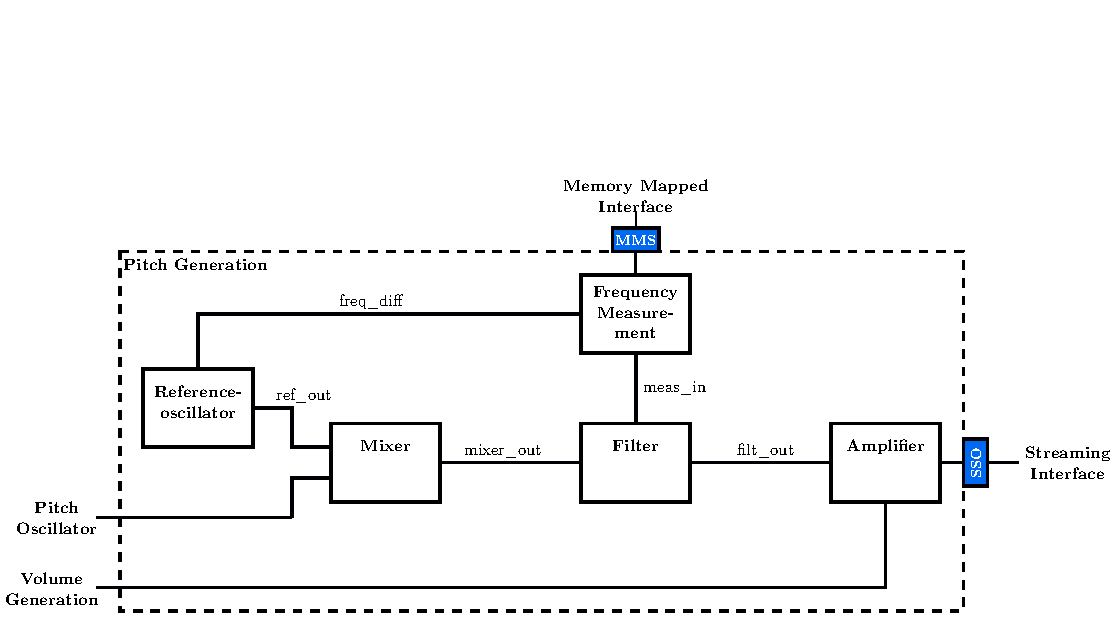
\includegraphics[width=1\textwidth]{Blockschaltbild_pitch.pdf}
	\caption{Blockschaltbild der Custom IP Pitch Generation} 
	\label{img:Blockschaltbild_pitch}
\end{figure}  



\paragraph{Referenzoszillator}

Der Referenzoszillator ist wie in Kapitel ... \todo{Referenz auf Grundlagen digitales Theremin} dafür zuständig ein Sinussignal mit Einer Frequenz ähnlich wie der Antennenoszillator ui generieren. Er generiert diesen wie schon erwähnt mithilfe des Cordic Algorithmus. Er ist aufgeteilt in zwei Komponenten: der Cordic Processor und der Cordic Controller. Wie diese beiden Komponenten miteinander verbunden sind ist in Abbildung \ref{img:Referenceoscillator} ersichtlich. \\

Der Cordic Processor berechnet einen Sinuswert aus ...

Der Cordic Controller berechnet den Winkelwert phi in der Form von Abbildung ... \todo{referenz Bild phi einfügen}. 

\begin{figure}[h!]
	\centering
	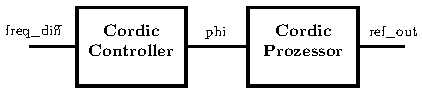
\includegraphics[width=0.53\textwidth]{Referenceoscillator.pdf}
	\caption{Aufbau des Referenzoszillators} 
	\label{img:Referenceoscillator}
\end{figure}  

\todo{Bild phi einfügen}

\paragraph{Filter}

\begin{figure}[h!]
	\centering
	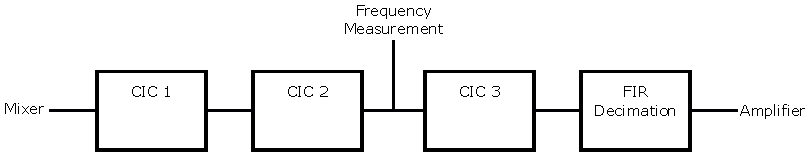
\includegraphics[width=1\textwidth]{Filter_pitch.pdf}
	\caption{Aufbau des Filters in der Komponente Pitch Generation} 
	\label{img:Filter_Pitch}
\end{figure}  

\paragraph{Frequenzmessung, Kalibration \& Glissandoeffekt}

Die Komponente Frequency Measurement hat mehrere Aufgaben und ist diejenige Komponente mit welcher über den Nios Prozessor die gesammte Pitch Generation gesteuert werden kann. Der Aufbau dieser Komponente ist in Abbildung \ref{freq_meas_pitch} aufgezeigt.\\
Zum einen wird hier die Frequenzmessung durchgeführt. Dies geschieht über die drei Komponenten FIR, Period Counter und Goldschmidt divider. FIR ist wie der Name sagt ein FIR Filter. Dieses ist nötig um das Signal aus dem Filter, welches noch Hochfrequente Signale enthält zu Filtern. Das Filter hat eine Grenzfrequenz von ... \todo{Grenzfrequenz und Dämpfung einfügen}. Das Filter wurde mit dem Tool filterDesigner in Matlab berechnet. Wir haben entschieden die Filterkoeffizienten als fixed-point signed Zahlen in einem Array mit \SI{18}{bit} länge abzuspeichern. Auf dieser Koeffizientenlänge kann Quartus die DSP-Blöcke so nutzen, dass nach der Multiplikation des Signals mit den Koeffizienten die Resultate gleich in den Blöcken addiert wird. Dies ermöglicht längereMultiplikationsketten. \todo{Nochmal über DSP blöcke nachlesen und referenzieren} \\
Anschliessend wird das Signal \textit{fir_out} im \textit{Period Counter ausgemessen}. Diese zählt von Nulldurchgang zu Nulldurchgang einen Zähler hoch. Bei einem Nulldurchgang wird der Wert dieses Zählers am Signal \textit{per_cnt} ausgegeben. Der Zählerwert entspricht der Anzahl Abtastwerte des Signals in einer Signalperiode. \\
Das Signal hat eine Abtastfrequenz von \SI{1.2}{MHz}. Dividiert man diese Abtastfrequenz durch die zuvor gezählte Anzahl Abtastperioden erhält man die Frequenz des Signals.

\begin{figure}[h!]
	\centering
	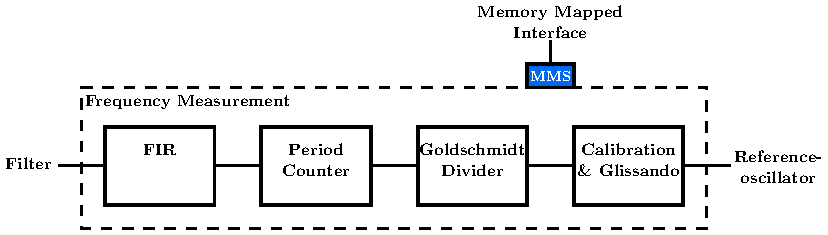
\includegraphics[width=1\textwidth]{freq_meas_pitch.pdf}
	\caption{Aufbau der Frequenzmessung, Kalibration und Glissandoeffekt in der Komponente Pitch Generation} 
	\label{img:freq_meas_pitch}
\end{figure}  
\todo{Bild überarbeiten und namen an Signalen anbringen wie in Text}